%%%%%%%%%%%%%%%%%%%%%%%%%%%%%%%%%%%%%%%%%
% "ModernCV" CV and Cover Letter
% LaTeX Template
% Version 1.1 (9/12/12)
%
% This template has been downloaded from:
% http://www.LaTeXTemplates.com
%
% Original author:
% Xavier Danaux (xdanaux@gmail.com)
%
% License:
% CC BY-NC-SA 3.0 (http://creativecommons.org/licenses/by-nc-sa/3.0/)
%
% Important note:
% This template requires the moderncv.cls and .sty files to be in the same
% directory as this .tex file. These files provide the resume style and themes
% used for structuring the document.
%
%%%%%%%%%%%%%%%%%%%%%%%%%%%%%%%%%%%%%%%%%
% 最后更新:2014年10月11日
%----------------------------------------------------------------------------------------
%   PACKAGES AND OTHER DOCUMENT CONFIGURATIONS
%----------------------------------------------------------------------------------------

\documentclass[10pt,a4paper,sans]{moderncv} % Font sizes: 10, 11, or 12; paper sizes: a4paper, letterpaper, a5paper, legalpaper, executivepaper or landscape; font families: sans or roman
% moderncv version 1.5.1 (29 Apr 2013)

\moderncvstyle{banking} % CV theme - options include: 'casual' (default), 'classic', 'oldstyle' and 'banking'
\moderncvcolor{black} % CV color - options include: 'blue' (default), 'orange', 'green', 'red', 'purple', 'grey' and 'black'

\usepackage[noindent]{ctex} %中文支持
% \setCJKmainfont{Libian SC}
\setCJKmainfont{Hannotate SC}

%\usepackage{lipsum} % Used for inserting dummy 'Lorem ipsum' text into the template

\usepackage[top=1cm,bottom=1.5cm,left=2cm,right=2cm]{geometry} % Reduce document margins
%\setlength{\hintscolumnwidth}{3cm} % Uncomment to change the width of the dates column
%\setlength{\makecvtitlenamewidth}{10cm} % For the 'classic' style, uncomment to adjust the width of the space allocated to your name

%----------------------------------------------------------------------------------------
%   NAME AND CONTACT INFORMATION SECTION
%----------------------------------------------------------------------------------------
\name{代}{岩}
% All information in this block is optional, comment out any lines you don't need
\title{个人简历}
\address{维多利亚大学}{惠灵顿, 新西兰}
\phone[mobile]{(+86)~136~83047987}
\email{alvin\_daiyan@hotmail.com}
\homepage{alvindaiyan.github.io}
%\social[twitter]{username}
\social[github]{alvindaiyan}
%\extrainfo{additional information}
%\photo[70pt][0.4pt]{photo} % The first bracket is the picture height, the second is the thickness of the frame around the picture (0pt for no frame)
%\quote{"A witty and playful quotation" - John Smith}

%----------------------------------------------------------------------------------------

\begin{document}

\makecvtitle % Print the CV title

%----------------------------------------------------------------------------------------
%   POSITION APPLIED(CAREER OBJECTIVE)
%----------------------------------------------------------------------------------------
\section{求职意向}
%\subsection{求职意向}
\cventry{期望月薪:  面议}{应聘职位:高级软件工程师}{}{}{}{}


%----------------------------------------------------------------------------------------
%   SKill Set
%----------------------------------------------------------------------------------------

\section{我的技术栈}

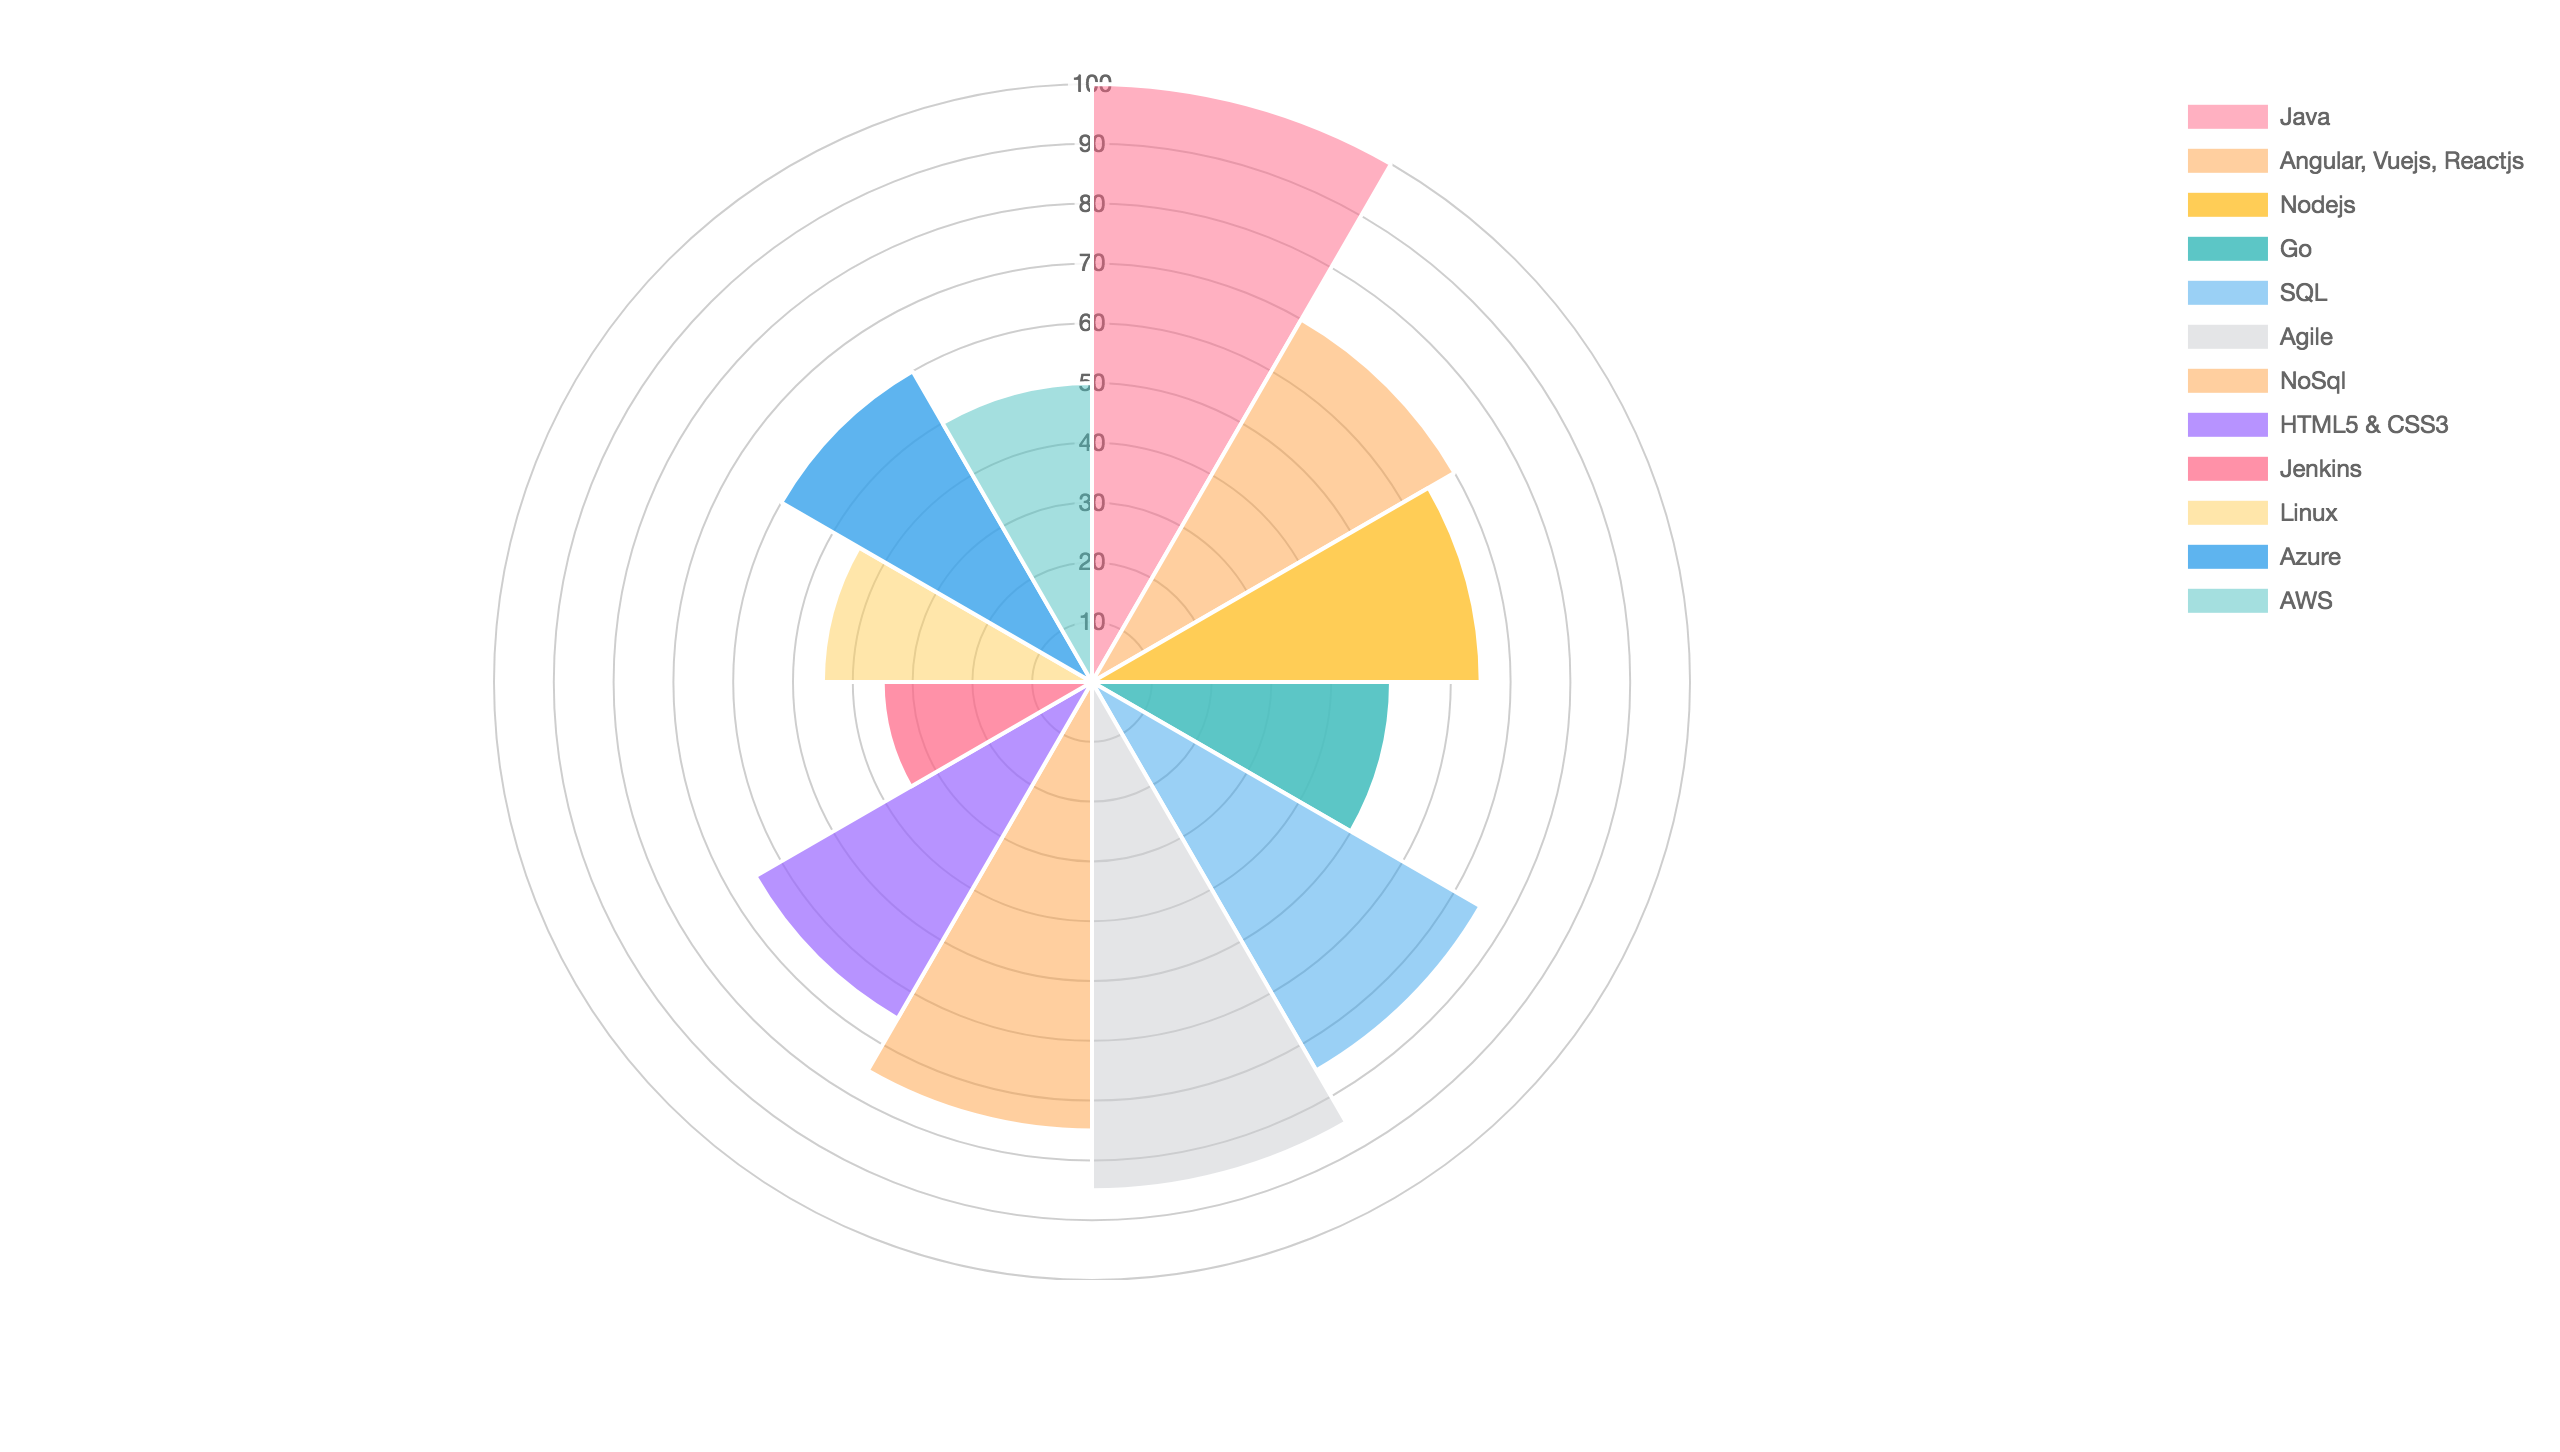
\includegraphics[width=\linewidth]{myskillset.png}
%----------------------------------------------------------------------------------------
%   EDUCATION SECTION
%----------------------------------------------------------------------------------------

\section{教育背景}

\cventry{2009---2013}{软件工程}{惠灵顿维多利亚大学}{本科}{}{}{\textit{GPA: 3.33/5(相当于百分制80分)}、惠灵顿大学荣誉学士}  % Arguments not required can be left empty

%----------------------------------------------------------------------------------------
%   WORK EXPERIENCE SECTION
%----------------------------------------------------------------------------------------

\section{项目经历}
%------------------------------------------------
\subsection{Department of Internal Affairs (新西兰内政部)}

\cventry{2017.05---现在}{主要项目成员,devops}{政府公共服务转型项目}{}{}{
\begin{itemize}
\setlength{\itemindent}{2em}
    \item 针对devops设计并搭建开发平台,编写基于Azure Resource Manager template自动化脚本
    \item 设计并开发基于Visual Studio Team Service的pipeline开发,通过pipline自动化部署Azure resource
    \item 设计并开发婚姻申请系统,前端:angular2,后端:nodejs,swagger等,数据库:cosmosdb(mongodb)
    \item 设计并开发出生证明申请系统,前端:angular5,后端:java8,springboot等
    \item 开发基于protractor和cucumber的自动化开发框架
    \item 参与code review,设计开发git flow,技术服务支持
%    \item 推行Go在政府到普及
\end{itemize}
}

%%------------------------------------------------
\subsection{iPayroll Ltd (iPayroll 有限公司)}

\cventry{2016.01---2017.05}{Java开发}{工资单系统}{}{}{
\begin{itemize}
\setlength{\itemindent}{2em}
    \item 维护基于java,spring,postgresql的工资单系统,系统年处理工资30亿纽币,在新西兰有8000企业用户
    \item 针对客户需求,开发新的功能
    \item 设计并开发基于restful的API和java sdk,文档可见于:http://dev.ipayroll.co.nz/
    \item 开发Timelog系统用于记录员工作时间,系统基于Angular1.4,spring
    \item 带领前端团队针对reactjs,angular2和vuejs的研究和技术选型
    \item 参与code review,设计开发git flow,技术服务支持
\end{itemize}
}

%%------------------------------------------------
\subsection{Syl Limited (Syl 有限公司)}

\cventry{2013.11---2015.12}{Java开发}{企业文档搜索引擎}{}{}{
\begin{itemize}
\setlength{\itemindent}{2em}
    \item 维护基于java,spring,cassandra,nlp的企业级搜索引擎
    \item 开发并部署上线针对IBM LotusNotes的java爬虫,并成功优化爬虫使其运行效率翻倍
    \item 设计并开发从MS Word,Excel和Powerpoint中提取嵌入式文档的模块(基于Java,apache POI),模块已运行于syl 2.1和syl 2.5平台。
    \item syl 2.1和syl 2.5平台的WordPerfect文档解析功能的主要开发者
    \item 开发syl 2.1和syl 2.5平台中元数据RESTful API(使用Jersey的JAX-RS)
\end{itemize}
}
%%------------------------------------------------
\subsection{北京神舟航天软件技术有限公司}

\cventry{2011.10---2012.3}{实习Java开发}{知识工程系统}{}{}{
\begin{itemize}
\setlength{\itemindent}{2em}
    \item 关于知识汲取,知识评估,知识评估等需求分析
    \item 开发在线pdf文档功能
    \item 研究有关贝叶斯算法,遗传算法和支持向量机等大数据系统用于自动错误发现系统
\end{itemize}
}
%%------------------------------------------------

%%------------------------------------------------
\subsection{Fronde Systems Group (Fronde 有限公司)}

\cventry{2013.01---2013.3}{实习Java开发}{自动账单计算系统}{}{}{
\begin{itemize}
\setlength{\itemindent}{2em}
    \item 分析,设计及实现复杂的收费规则
    \item 作为敏捷开发的scrum master,领导团队日常工作
    \item 设计与开发集成测试
\end{itemize}
}
%%------------------------------------------------
%----------------------------------------------------------------------------------------
%   AWARDS SECTION
%----------------------------------------------------------------------------------------

\section{荣誉奖励}
\cvitem{2013.11}{惠灵顿维多利亚大学荣誉学士}
\cvitem{2012.11}{惠灵顿维多利亚大学暑期奖学金项目}
\cvitem{2013.06}{于GECCO'13发表PSO for Feature Construction and Binary Classification}
\cvitem{2010}{在Habitat for Humanity做志愿者帮助开发慈善系统}

%----------------------------------------------------------------------------------------
%   AWARDS SECTION
%----------------------------------------------------------------------------------------

\section{个人爱好}
\cvitem{体育运动}{足球,篮球,乒乓球,羽毛球}
\cvitem{科技}{阅读科技类博客,写博客}
\cvitem{开源项目}{乐于在github上参与各种开源软件开发和贡献代码}


\section{语言}
\cvitem{英语}{流利口语及书写}
\end{document}
